%!TEX root=../thesis.tex
\chapter{Experiments} \label{cha:experiments}

This chapter outlines all the methodologies used to analyze the test application
and it provides a discussion of the outcomes.


\section{First measurements}\label{sec:first_measurements}
The first step to outline the behaviour of the test application is to include
the the Web Tracing Framework library and to place the proper functions in the
source code as shown in Listing \ref{code:wtf_example}.
Consequently, the profiling measurements are obtained following the
metodologies explained in Sections \ref{sec:assumptions} and \ref{sec:procedure}.

This very first approach can be considered as an
exploratory phase. If all the default events available to the WTF are enabled, the
resulting trace contains a considerable amount of data. Fortunately there is a
graphical interface that allows to easily navigate the hierarchical structure
of the function calls inside the trace. After understanding the data format,
a selection of the interesting function calls is outlined for
restricting the search field only to WebGL functions. The resulting list of primitives
is presented in Table \ref{tab:webgl_function_list}.
\begin{table}[!htb]
    \centering
    \caption{The list of the WebGL function of interest.}
    \label{tab:webgl_function_list}
    \begin{tabular}{|lllll|}
        \hline
        bindBuffer    & viewport        & clearColor    & bindTexture & uniformMatrix4v \\
        bufferSubData & clear           & createTexture & pixelStorei & linkProgram     \\
        disable       & bindFrameBuffer & activeTexture & textImage2D & \\
        \hline                
    \end{tabular}
\end{table}

After some preliminary test, the trace extracted from the ``no-map'' scenario
is selected as the first to be analyzed in detail. This choice is made
to clarify the potential of the framework and to understand its limits, since
this is the basic building block for the rest of the work.
Profiling the navigator in the abovementioned scenario results in a trace that
illustrates a very interesting result. Figure \ref{img:no_map_overview}
shows a timeline representation of the trace, where every colored vertical bar
symbolizes the occurrence of a function call or an event tracked by the tool.
As it is possible to notice, all of them are arranged into fairly regular groups.
\begin{figure}[!htb]
    \center{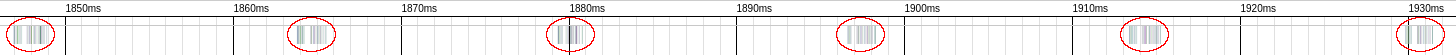
\includegraphics[width=1\linewidth]{no_map_overview.png}}
    \caption{An example trace highlighting the function groups.}
    \label{img:no_map_overview}
\end{figure}

Furthermore, it turns out that every group always start with a \emph{bindBuffer}
call. According to the WebGL official documentation\footnote{
\url{https://developer.mozilla.org/it/docs/Web/API/WebGL_API}.}, this function is
responsible for binding a buffer object containing vertexes and/or colors to the
current WebGL context. Essentially it marks an arbitrary buffer to be the current
one where all the other WebGL functions will work on. This is necessary due to the
inability of the GPU process to deal with more than one data structure at a time.
Hence, it allows to virtually split the trace into small groups by means of the
\emph{bindBuffer} function calls.

After identifying the particular structure underlying the trace, it is possible to check
which are the recurrent WebGL functions belonging to each group (ie. the red ellipses
in Figure \ref{img:no_map_overview}) and to gather them into macro-operations sets.
If a check about the specific task fulfilled by each WebGL function is performed, it
becomes clear that they belong to the three following main scopes:
\begin{itemize}
    \item \emph{initialization/load data}: every WebGL function in this group
        is responsible for preparing the data structures loaded in memory
        and for copying all the needed data (eg. copies the bitmap of a texture
        to the proper buffer).
    \item \emph{modify data}: these functions actually work on the vertex/color
        buffer to modify the data contained in it, especially via matrix
        operations (eg. updates the value for a subset of objects in the buffer
        according to some linear transformation).
    \item \emph{display/draw}: this group is the one sending the commands
        that are actually used by the GPU to draw the shapes on the screen
        (eg. renders the vertexes stored in a buffer to build more complex shapes).
\end{itemize}

A more detailed functions-to-groups mapping is outlined in Table
\ref{tab:webgl_func_mapping}.

\begin{table}[!htb]
    \centering
    \caption{WebGL functions-to-groups mapping.}
    \label{tab:webgl_func_mapping}
    \begin{tabular}{|l|l|l|}
        \hline
        \textbf{Initialization/load data} & \textbf{Modify data} & \textbf{Display/draw} \\ \hline
        bindBuffer/bindFramebuffer & uniformMatrix3fv/uniformMatrix4fv & drawElements \\
        enable/disable & uniform[1\(\vert\)2\(\vert\)3\(\vert\)4][f\(\vert\)i\(\vert\)iv\(\vert\)fv] & drawArrays \\
        viewport & bindTexture/activeTexture &  \\
        clear/clearColor & bufferSubData &  \\
        cullFace &  &  \\
        depthCompare &  &  \\
        useProgram &  &  \\
        colorMask &  &  \\
        \hline
    \end{tabular}
\end{table}

Another important aspect is to realize if and how the values of the timings fluctuate 
during a run of the application.
As it is possible to see from Figure \ref{img:no_map_example},
there can be outliers where the response time is significantly larger with respect
to the rest of the trace.
\begin{figure}[!htb]
    \center{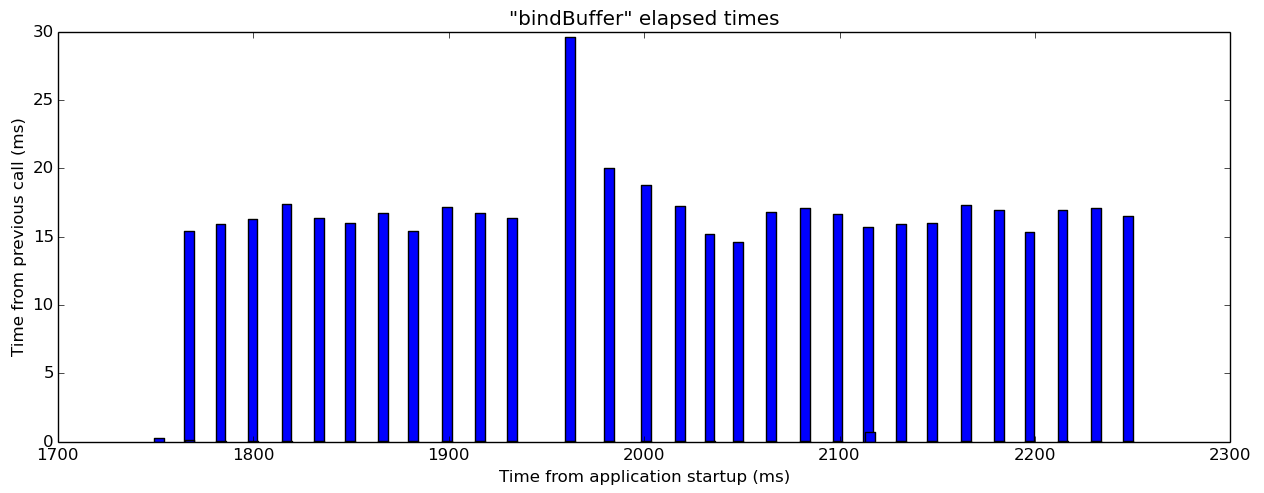
\includegraphics[width=0.75\linewidth]{500ms_1_no_map.png}}
    \caption{A trace extracted from the ``no-map'' scenario.}
    \label{img:no_map_example}
\end{figure}

This fluctuating trend can have several justifications which need to be investigated
further. Since this framework is able to measure only the response times of the application
with a precision of \(\pm 0.5\,ms\), the bar chart shown in Figure
\ref{img:no_map_example} displays a compounded value on the Y axis. The response
time can be described as follows:
\begin{equation}
    response\_time = computation\_time + interference
    \label{eq:response_time}
\end{equation}

The \emph{interference} component is clearly due to the huge operating system
stack lying between the JavaScript code, running inside the
browser, and the Mesa 3D graphics driver, which is part of the Linux OS kernel.
Hence, this inconvenience needs to be reduced as much as possible in order not
to jeopardize the validity of the results presented in this chapter.
One possibility to mitigate
the interference from higher priority tasks is to increase that of
the Googhe Chrome instance using the \emph{nice}\footnote{\url{https://linux.die.net/man/1/nice}.}
tool. Another approach includes directly changing the scheduling policy via the
\emph{chrt}\footnote{\url{http://man7.org/linux/man-pages/man1/chrt.1.html}.}
utility for using a different scheduling algorithm. After several attempts,
it is possible to state that no
noteworthy difference in the response times can be observed after applying these
methods. For this reason, further investigations regarding the \emph{computation\_time}
component are foundamental for better studying these fluctuations.

Moreover, after dividing all the WebGL functions into macro-operations groups
(see Table \ref{tab:webgl_func_mapping}) it is possible to refine the graph shown
in Figure \ref{img:no_map_example}. As it is possible to see from Figure
\ref{img:no_map_groups}, this ``grouped'' bar chart is very useful to understand
the weight of every set of operations with respect to the time elapsed between
each \emph{bindBuffer} function call.
\begin{figure}[!htb]
    \center{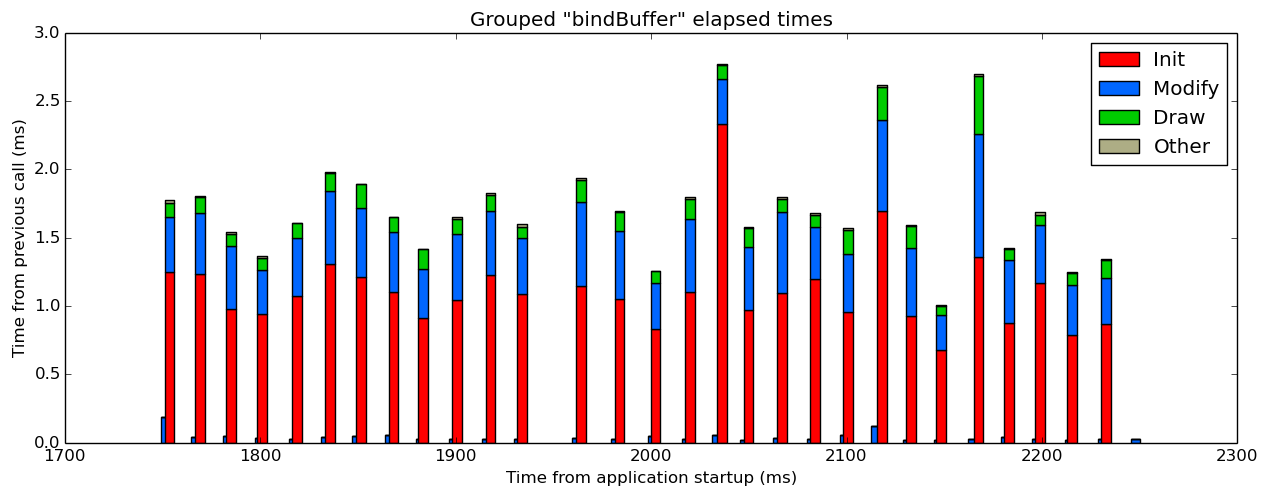
\includegraphics[width=0.8\linewidth]{500ms_1_no_map_groups.png}}
    \caption{An example of a grouped bar chart computed from a trace.}
    \label{img:no_map_groups}
\end{figure}

Finally, a comparison between extensive 2D and 3D tests showed that response times
during 3D rendering are slightly higher and more prone to fluctuations. This is
certainly due to the different computation workloads which can significantly change
over time, depending on the complexity of the scene to be rendered.
This analysis using the WTF allows to outline an approximate model, where
each job of the rendering task can be divided into three logically different
parts. This finding can be graphically summarized as shown in Figure \ref{img:call_arrival}.
\begin{figure}[!htb]
    \center{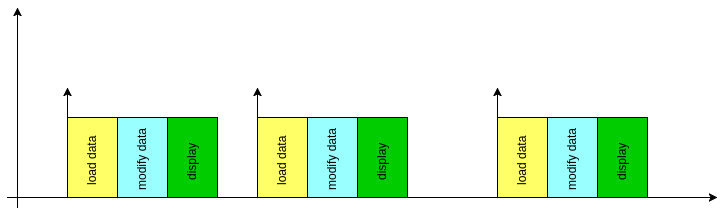
\includegraphics[width=0.6\linewidth]{call_arrival.png}}
    \caption{The graphics functions arrival approximate model with the different groups.}
    \label{img:call_arrival}
\end{figure}


\section{A fine-grained model}
Some other approach is needed to get better insights with respect to the ones
presented in the previous chapter. The WTF is able to retrieve only response
times (see Equation \ref{eq:response_time}) but, usually, real-time models
deal with computation times.
Hence, the problem of measuring exact computation
times without the interference coming from other tasks becomes a strict requirement.
Another important aspect is the resolution of the timings. As stated in Section
\ref{sec:first_measurements}, the Web Tracing Framwork is able to extract times with a
\( \pm 0.5\,ms \) precision and it is clearly not enough for applying any of
the real-time mathematical models presented in the literature.
Last but not least, a more fine-grained view of the function calls involved in
the rendering process is required. This allows to focus only on the
``\emph{display/draw}'' group presented in Table \ref{tab:webgl_func_mapping},
without restricting the analysis to the \emph{drawElements} and \emph{drawArrays}
functions found by the WTF. To some extent, another way to dig deeper into the
WebGL technology is needed for realizing what happens at the core level of the
web browser.

It immediately become clear that the tool presented in Section \ref{sec:first_measurements}
is not powerful enough to recognize what is happening inside the browser internals.
The tool that perfectly fits these requirements is the \emph{Trace Event Profiling
Tool}~\cite{eventprofilertool} embedded into the Chrome web browser.
It allows to capture computation times (and not only response times) of multiple
events, including the ones handled by the GPU process. Being able to distinguish
the \emph{computation\_time} from the \emph{interference} component is the key
that permits to apply mathematical models that would not be possible otherwise.
To be more precise, for the purpose of this thesis,
the profiler enables to captures the ``duration events'' of the commands received by the GPU
process from a server-side point of view (and not from the renderer client perspective).
Moreover it achieves more precise timings with a resolution of \(\pm 1\,\mu s\),
which is three orders of magniture greater than the one of WTF.
Finally, this event tracing tool is able to accurately trace which are the functions
being called inside the Chrome's source code and to identify the object's class
calling that method. Therefore, it is possible to say that it is able to perfectly
balance the defects of the Web Tracing Framework.

The grouped bar chart displayed in Figure \ref{img:no_map_groups} helped to
get an idea about the wheight each group has inside the entire response time.
Since this thesis aims at modelling the rendering pipeline of WebGL from a real-time
point of view, the focus is put only to the ``\emph{display/draw}'' group.

The Trace Event Profiling Tool has been designed to diagnose performance problems,
allowing the developer to understand what the browser is doing ``under the hood''.
Due to the milti-process nature of Chrome, this toolkit is able to record
both the activity of each Chrome's process and the proper method signatures
(from the C++ core up to the client's JavaScript code). This procedure results in
a huge amount of information, which can be visually inspected with a graphical
interface or it can be exported in JSON format for successive automatic analysis
tasks.

Another important aspect is how this tool is meant to be used in practice. The normal use case
works as follows. First, open a new tab for the tool typing \url{about://tracing}
insede the URL bar.
Next click the ``record'' button to select only the events of interest and to
start capturing a trace. After that, switch to the tab with the target content
to be debugged and perform each operation needed to reproduce the bug or to trigger
the code behaving incorrectly. Once the scenario has been triggered, switch back to the profiler
tab, click the ``stop'' button and wait until the tool extracts all the needed
information to build the GUI. Finally, the trace can be either inspected directly
from the tool's web interface (see Figure \ref{img:chrome_profiler}) or it can be
exported to a JSON file via the ``save'' button.
\begin{figure}[!htb]
    \center{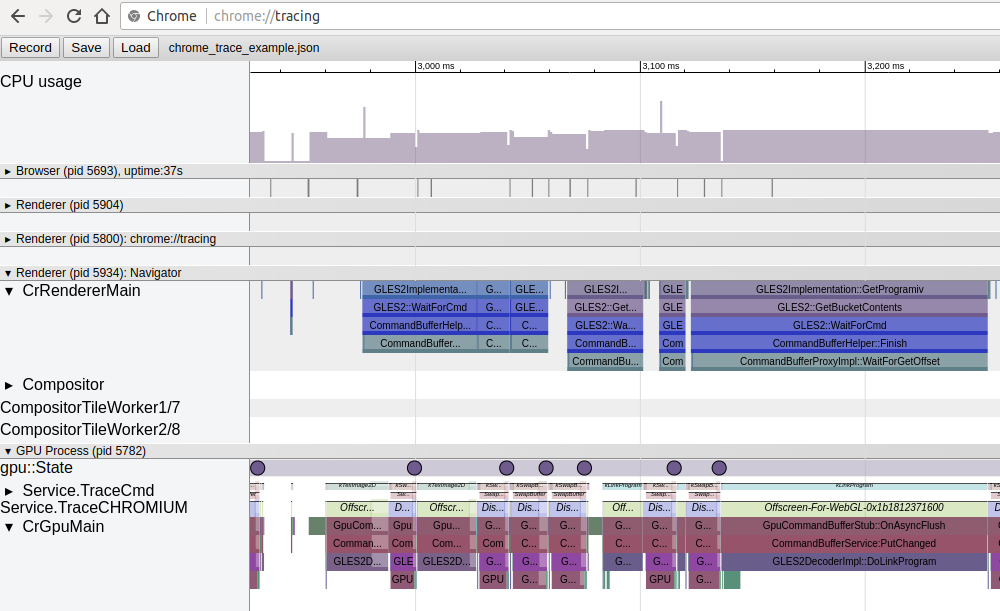
\includegraphics[width=0.65\linewidth]{chrome_profiler_screenshot.png}}
    \caption{A trace inspection using the Trace Event Profiling Tool interface.}
    \label{img:chrome_profiler}
\end{figure}

Sometimes, it may be necessary to run Chrome with some specific command
line parameter for enabling specific benchmarking options that would not be
available by default\footnote{These special command line options allow to trace
events that would not be fired otherwise, since the vast majority of Chrome's
users do not need them and they prefer a smoother navigation experience. A complete
list of all the command line switches is available at
\url{https://peter.sh/experiments/chromium-command-line-switches/}.}.
For example, the \emph{-{}-enable-skia-benchmarking} flag is needed to enable the
code instrumentation for the Skia graphics engine of the browser, which allows
this tool to capture also the events created by that specific
component of the web browser.


\subsection{Trace capturing}
Among all the information about the Event Trace Profiling tool itself presented
in the previous section, it is
also important to understand the scenario where the traces analyzed in Section
\ref{sec:math_model} are captured.

The traces displayed in~\cite{frias2017probabilistic} represent the computation
times of a lane detection algorithm~\cite{fontanelli2014vision} used by a robot
to determine its position with respect to some line markers arranged on the floor.
More specifically, it takes as input an image and it outputs ``the distance
of the center of the vehicle from the line and the angle between the longitudinal
axis of the car and the line''. Such algorithm samples the \emph{relevant elements}
from the frame in order to detect the line and to allow the robot to move accordingly.
It follows that the so called relevant elements are not always the same throughout
all the images captured by the camera.

In order to mimic this random component in the test application presented in this
thesis, the starting point of the navigation (ie. latitude and longitude) and
the rotation of the camera are taken randomly at each run.
This means that it is not possible to know in advanche the path followed on the
map, thus ensuring the unpredictability of the computation times of the WebGL
rendering pipeline.

Furthermore, among all the information captured by the
Chrome's Event Trace Profiling Tool, only data concerning the GPU process is
extracted. This allows to retrieve not only the timestamps of the events (ie.
response times), but also the more relevant duration of complete events using
the \emph{tdur} field. This value specifies the thread clock duration of complete
events in microseconds, which corresponds to the computation times.


\section{The mathematical model}\label{sec:math_model}
Generally speacking, a real-time task \(\tau_{i}\) is composed of multiple jobs
\(J_{i,\,j}\) which activate at time \(r_{i,\,j}\), finish at time \(f_{i,\,j}\)
and compute for an amount of time \(c_{i,\,j}\). The real-time models in the
literature the computation time \(c_{i\,j}\) as an i.i.d. stochastic process \(C\).
On the contrary, the model presented in~\cite{frias2017probabilistic} is not
based on this tightening assumption. In addition, probabilistic
deadlines~\cite{abeni1999qos} are used instead of the normal hard ones.
This approach to real-time modeling techniques has been developed because the
computation times studied by Fr\'{i}as et at. in~\cite{frias2017probabilistic}
are strongly correlated with the previous ones and do not respect the i.i.d.
assumption. Another notheworthy aspect of these computation times is that they
are random even for multiple executions of the same task on the same input data.
Moreover, the lane algorithm presents a ``switching behaviour'', since computation
times can change considerably depending on the scene taken as input.

Hence, this scenario does not allow to describe all the computation times with
a unique probability distribution but, at the same time, it has to be described
using some stochastic process. This is what the \emph{Markov Computation Time Model}
(MCTM) aims to solve.
The MCTM model works as follows. The switching behaviour of the computation
times stated above can be described as a system with a finite number of states
(\emph{N}). The computation time samples belonging to each state are represented
by a random process, which can be further described with its probability
distribution if the random process withstand to the i.i.d. assumption.
Moreover, if the transitions between the \emph{N} modes can be defined as a Markov
process, the model just presented is a particular type of non i.i.d. processes
named \emph{Markov Modulated Process} (MMP)~\cite{fischer1993markov}.
More precisely it is an Hidden Markov Model (HMM)~\cite{eddy1996hidden}, since
the only observable part is the output of each state (ie. the computation times)
and not the states themselves.

More formally, the MCTM is defined as a triple \(\{M,\,P,\,C\}\) where:
\begin{itemize}
    \item \( M = \{ m_1,\,\dots,\,m_N \} \) is the set of modes.
    \item \( P = (p_{a,\,b}) \) is the mode transition matrix, where
        \(a \in M\) and \(b \in M\).
    \item \( C = \{ C_{m_j} : m_j \in M \} \) is the set of probability
        distributions of the computation times for each mode.
\end{itemize}
